\documentclass[10pt]{beamer}

\usecolortheme{dove}
\definecolor{mycyan}{rgb}{0.2157, 0.7059, 0.9608}
\setbeamercolor{alerted text}{fg=mycyan}
\setbeamertemplate{bibliography item}{\insertbiblabel}
\setbeamertemplate{caption}[numbered]
\hypersetup{colorlinks,linkcolor=,urlcolor=mycyan}
\usepackage{animate,xcolor,colortbl,listings,nicefrac}
\usepackage[italian]{babel}

\usepackage{listings}
\lstset{upquote=false}
\usepackage[]{framed}
\begin{document}


\begin{frame}
  \title{GMRES}
  \subtitle{Metodo generalizzato dei minimi residui applicabile in un sottospazio di Krylov per la soluzione numerica di equazioni lineari non simmetriche.}
  \date{19/03/2020}
  \author[Principal]{Fabio Archenti \and Fabio Camagni \and Andrea Favero \and  \\Lorenzo Fiamingo \and Stefano Galivanone \and Nazariy Nashkolnyy}
  \maketitle
\end{frame}


\begin{frame}

La presentazione deve iniziare con la lista del materiale
bibliografico utilizzato. Questo è un esempio di come inserire 
un libro o un articolo nella bibliografia.
  \frametitle{Bibliografia}
  \begin{thebibliography}{99}\small
    
    \bibitem{quarteroni2012calcolo}
    Quarteroni, Saleri, and Gervasio.
    \newblock {\em Calcolo Scientifico: Esercizi e problemi risolti con MATLAB e  Octave}.
    \newblock UNITEXT. Springer Milan, 2012.

    \bibitem{Cagnoni2013}
    Cagnoni, Agostini, Christen, Parolini, Stevanovi{\'c}, and de~Falco.
    \newblock Multiphysics simulation of corona discharge induced ionic wind.
    \newblock {\em Journal of Applied Physics}, 114(23), 2013.

   \bibitem{africa2017simultaneous}
   Africa, de~Falco, Maddalena, Caironi, and Natali.
   \newblock Simultaneous extraction of density of states width, carrier mobility
   and injection barriers in organic semiconductors.
   \newblock {\em Scientific reports}, 7(1):1--11, 2017.

   \end{thebibliography}

Una volta inserito un documento in bibliografia, 
può essere citato così:~\cite{quarteroni2012calcolo}
  
\end{frame}  

\begin{frame}
  \frametitle{Sommario}
  Questo comando inserisce una lista delle sezioni in
  cui è divisa la presentazione. Perché una sezione appaia 
  nel sommario deve contenere almeno una pagina.
  \tableofcontents
\end{frame}

\section{Prima sezione}\label{sec:sec1}

\begin{frame} \frametitle{Come inserire una formula}
Una formula può essere inserita all'interno del testo così : 
$-\nabla \left( \varepsilon \nabla u \right) = f $ oppure 
centrata e numerata così:
\begin{equation}\label{eq:poisson}
    -\nabla \cdot \left( \varepsilon \nabla u \right) = f
\end{equation}
oppure centrata senza numerazione così :
$$
 -\nabla \cdot \left( \varepsilon \nabla u \right) = f
$$
Posso fare riferimento alle formule numerate così : \eqref{eq:poisson}
\end{frame}

\begin{frame} \frametitle{Come inserire una lista per punti}
Ecco come inserire una lista per puti
\begin{itemize}
    \item un punto
    \item un altro
\end{itemize}
oppure un elenco numerato
\begin{enumerate}
    \item primo punto
    \item secondo punto
\end{enumerate}

\end{frame}

\section{Seconda sezione}\label{sec:sec2}

\begin{frame} \frametitle{Come inserire un pezzo di codice}
Si può evidenziare \alert{parte del testo} in questo modo.
%
Si può inserire un comando matlab all'interno del testo
in questo modo : \lstinline[language=Matlab]{for i = 1 : 10, disp (i), end}

si può inserire un un file contenete un codice matlab in questo modo :
\lstinputlisting[language=Matlab]{codice.m}

Si possono inserire solo alcune righe del file in questo modo :
\lstinputlisting[language=Matlab, firstline=1, lastline=2]{codice.m}

\end{frame}

\section{Terza sezione}\label{sec:sec3}

\begin{frame} \frametitle{Come inserire una figura}
Questo è un esempio di come inserire una figura
\begin{figure}
    \centering
    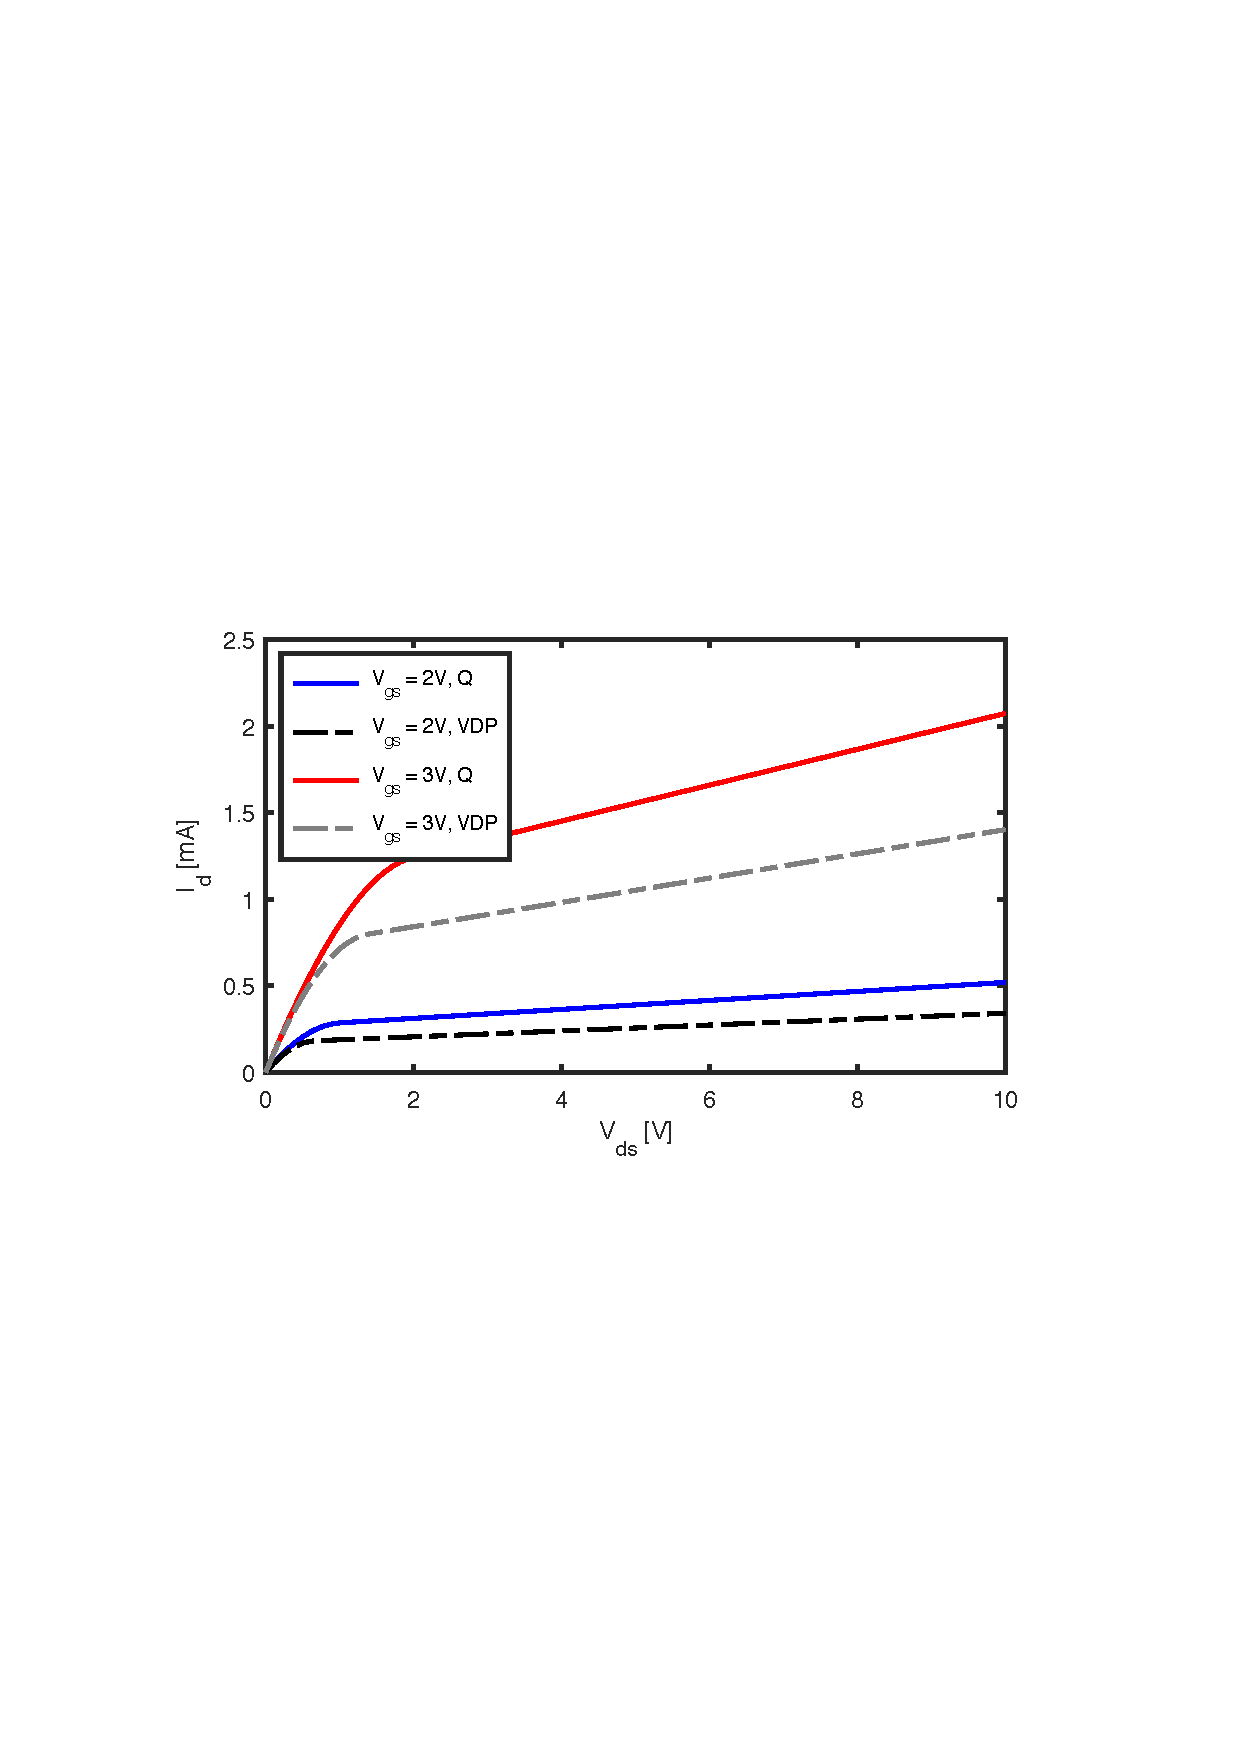
\includegraphics[width=.75\linewidth]{iv.pdf}
    \caption{Questa è la didascalia}
    \label{fig:my_label}
\end{figure}
Se la figura ha un'etichetta la si può usare per fare riferimento
alla figura nel testo : Figura~\ref{fig:my_label}
\end{frame}

\begin{frame} \frametitle{Altra documentazione}
Questo è un esempio di come inserire un link ad un URL
\begin{itemize}
    \item Altre informazioni utili
    \begin{itemize}
        \item Il sito del \href{https://www.latex-project.org}{\LaTeX{}--project}
            \begin{itemize}
                \item Una lista di 
                \href{https://www.latex-project.org/get}{software offline ed online}\\
                per creare documenti \LaTeX{}
            \end{itemize}
        \item Un \href{https://en.wikibooks.org/wiki/LaTeX}{Wikibook} su \LaTeX
        \begin{itemize}
            \item La sezione sulle \href{https://en.wikibooks.org/wiki/LaTeX/Presentations}
            {presentazioni}
            \item La sezione sulle
            \href{https://en.wikibooks.org/wiki/LaTeX/Mathematics}{formule}
        \end{itemize}
        \item Un \href{https://tex.stackexchange.com/}{forum} con domande e risposte
        \item La documentazione di \href{https://it.overleaf.com/learn}{overleaf}
        \begin{itemize}
            \item Un \href{https://it.overleaf.com/learn/latex/Learn_LaTeX_in_30_minutes}
            {tutorial} per iniziare in 30 minuti
        \end{itemize}
        \item Uno strumento per \href{http://detexify.kirelabs.org/classify.html}
        {cercare simboli}
    \end{itemize}
\end{itemize}
\end{frame}
\end{document}
